\newcommand{\walletcollector}{\texttt{wallet\_collector}}
\newcommand{\userinforetriever}{\texttt{user\_info\_retriever}}
\newcommand{\addresschecker}{\texttt{address\_checker}}
\newcommand{\graph}{\texttt{graph}}

\section{Nduja}
\subsection{High level architecture}
Nduja was developed in Python\footnote{it should be used with Python3.5+} and it
is composed by four main modules, represented in Figure\ref{fig:architecture}:
\begin{enumerate*}[label=\roman*),itemjoin={,\quad}]
\item \walletcollector{} is a set of classes whose aim is to retrieve
addresses of different cryptocurrencies. It provides a different class for each
different sources that we used, following the same interface
\item \userinforetriever{} is a set of classes that, based on which
site a wallet is discovered, retrieve some information (e.g. name, email,
personal website) related to the owner of that wallet
\item \addresschecker{} is a module that have to check if a sequence of
characters recognized as an address is a real and used addresses. For certain
altcoins it is not possible to perform this validation action accurately, e.g.
Monero has private transactions, so it is not possible to find out that
information
\item \graph{} is the module that create graph with which is possible to
correlate addresses and plot graphs.
\end{enumerate*}

\begin{figure}[H]
\centering
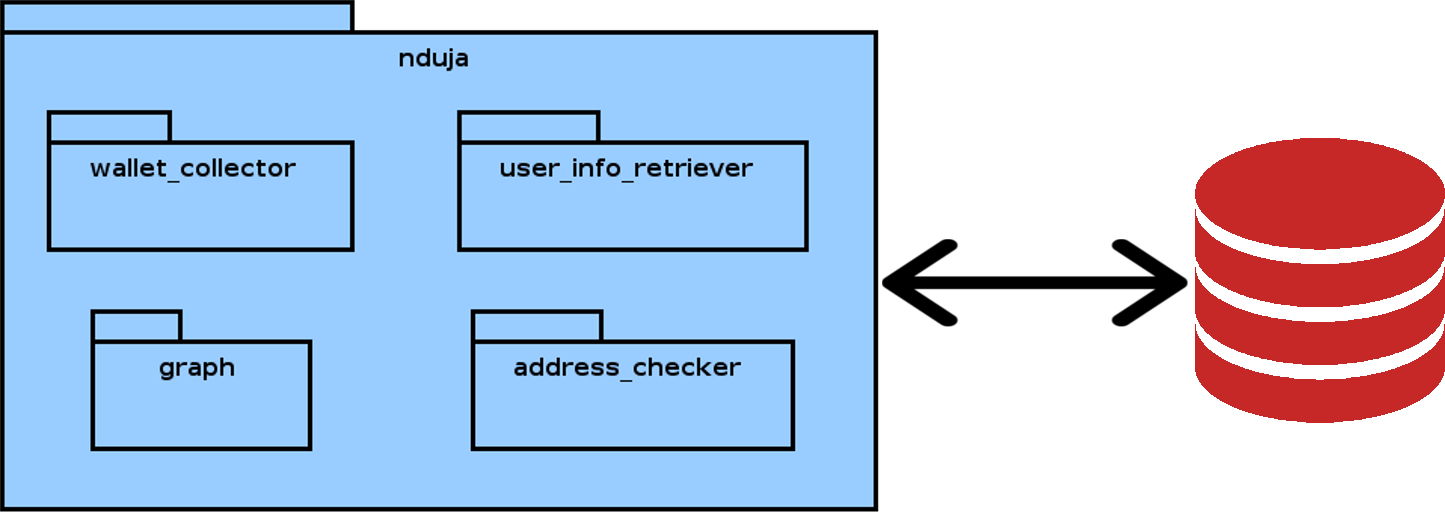
\includegraphics[scale=0.2]{db}
\caption{Nduja high level architecture}
\label{fig:architecture}
\end{figure}

\subsection{Queries} 
\label{sec:queries}
In order to maximize the number of possible results in repositories the module
\walletcollector{} searches for files that contains words such as
\textbf{donation} or \textbf{contribution} and in which there is a set of
characters that matches regular expressions that we defined for different
address formats. This has been implemented using two different APIs: Github
Search API \footnote{\url{https://developer.github.com/v3/search/}} and
Searchcode API \footnote{\url{https://searchcode.com/api/}}.
Instead, in order to query Twitter we looked for the same keywords that in the
repositories but also for \textit{hashtags} such as \textbf{\#GiveAway} or for
hashtags correlated to specific cryptocurrency (e.g. \#BTCGiveAway). This has
been done using Twitter API
\footnote{\url{https://developer.twitter.com/en/docs/api-reference-index}}.
Twitter API has a strong limitation: we are only able to retrieve tweets that
are published at most a week before the search. If there was a possibility to
bypass this limitation it could be possible to retrieve even more information.

\subsection{Database}
All data we have retrieved is stored into a
SQLite\footnote{\url{https://www.sqlite.org/}} database. Addresses are save with
the indication that if they are wallets retrieved from the websites we search,
if they are inferred or they are ``tagged'' addresses. These are wallets that
are known a priori: that means that are used by famous services, such as mixing
services or betting games as
\textit{SatoshiDICE}\footnote{\url{satoshidice.com}}. We excluded that kind of
services from data retrieving process for two reasons: the first is that we did
not want that the number of addresses explode, the latter is that these
addresses are ``public'' yet, so they are useless for the aim of our study.
